\documentclass[1p]{elsarticle_modified}
%\bibliographystyle{elsarticle-num}

%\usepackage[colorlinks]{hyperref}
%\usepackage{abbrmath_seonhwa} %\Abb, \Ascr, \Acal ,\Abf, \Afrak
\usepackage{amsfonts}
\usepackage{amssymb}
\usepackage{amsmath}
\usepackage{amsthm}
\usepackage{scalefnt}
\usepackage{amsbsy}
\usepackage{kotex}
\usepackage{caption}
\usepackage{subfig}
\usepackage{color}
\usepackage{graphicx}
\usepackage{xcolor} %% white, black, red, green, blue, cyan, magenta, yellow
\usepackage{float}
\usepackage{setspace}
\usepackage{hyperref}

\usepackage{tikz}
\usetikzlibrary{arrows}

\usepackage{multirow}
\usepackage{array} % fixed length table
\usepackage{hhline}

%%%%%%%%%%%%%%%%%%%%%
\makeatletter
\renewcommand*\env@matrix[1][\arraystretch]{%
	\edef\arraystretch{#1}%
	\hskip -\arraycolsep
	\let\@ifnextchar\new@ifnextchar
	\array{*\c@MaxMatrixCols c}}
\makeatother %https://tex.stackexchange.com/questions/14071/how-can-i-increase-the-line-spacing-in-a-matrix
%%%%%%%%%%%%%%%

\usepackage[normalem]{ulem}

\newcommand{\msout}[1]{\ifmmode\text{\sout{\ensuremath{#1}}}\else\sout{#1}\fi}
%SOURCE: \msout is \stkout macro in https://tex.stackexchange.com/questions/20609/strikeout-in-math-mode

\newcommand{\cancel}[1]{
	\ifmmode
	{\color{red}\msout{#1}}
	\else
	{\color{red}\sout{#1}}
	\fi
}

\newcommand{\add}[1]{
	{\color{blue}\uwave{#1}}
}

\newcommand{\replace}[2]{
	\ifmmode
	{\color{red}\msout{#1}}{\color{blue}\uwave{#2}}
	\else
	{\color{red}\sout{#1}}{\color{blue}\uwave{#2}}
	\fi
}

\newcommand{\Sol}{\mathcal{S}} %segment
\newcommand{\D}{D} %diagram
\newcommand{\A}{\mathcal{A}} %arc


%%%%%%%%%%%%%%%%%%%%%%%%%%%%%5 test

\def\sl{\operatorname{\textup{SL}}(2,\Cbb)}
\def\psl{\operatorname{\textup{PSL}}(2,\Cbb)}
\def\quan{\mkern 1mu \triangleright \mkern 1mu}

\theoremstyle{definition}
\newtheorem{thm}{Theorem}[section]
\newtheorem{prop}[thm]{Proposition}
\newtheorem{lem}[thm]{Lemma}
\newtheorem{ques}[thm]{Question}
\newtheorem{cor}[thm]{Corollary}
\newtheorem{defn}[thm]{Definition}
\newtheorem{exam}[thm]{Example}
\newtheorem{rmk}[thm]{Remark}
\newtheorem{alg}[thm]{Algorithm}

\newcommand{\I}{\sqrt{-1}}
\begin{document}

%\begin{frontmatter}
%
%\title{Boundary parabolic representations of knots up to 8 crossings}
%
%%% Group authors per affiliation:
%\author{Yunhi Cho} 
%\address{Department of Mathematics, University of Seoul, Seoul, Korea}
%\ead{yhcho@uos.ac.kr}
%
%
%\author{Seonhwa Kim} %\fnref{s_kim}}
%\address{Center for Geometry and Physics, Institute for Basic Science, Pohang, 37673, Korea}
%\ead{ryeona17@ibs.re.kr}
%
%\author{Hyuk Kim}
%\address{Department of Mathematical Sciences, Seoul National University, Seoul 08826, Korea}
%\ead{hyukkim@snu.ac.kr}
%
%\author{Seokbeom Yoon}
%\address{Department of Mathematical Sciences, Seoul National University, Seoul, 08826,  Korea}
%\ead{sbyoon15@snu.ac.kr}
%
%\begin{abstract}
%We find all boundary parabolic representation of knots up to 8 crossings.
%
%\end{abstract}
%\begin{keyword}
%    \MSC[2010] 57M25 
%\end{keyword}
%
%\end{frontmatter}

%\linenumbers
%\tableofcontents
%
\newcommand\colored[1]{\textcolor{white}{\rule[-0.35ex]{0.8em}{1.4ex}}\kern-0.8em\color{red} #1}%
%\newcommand\colored[1]{\textcolor{white}{ #1}\kern-2.17ex	\textcolor{white}{ #1}\kern-1.81ex	\textcolor{white}{ #1}\kern-2.15ex\color{red}#1	}

{\Large $\underline{12a_{0613}~(K12a_{0613})}$}

\setlength{\tabcolsep}{10pt}
\renewcommand{\arraystretch}{1.6}
\vspace{1cm}\begin{tabular}{m{100pt}>{\centering\arraybackslash}m{274pt}}
\multirow{5}{120pt}{
	\centering
	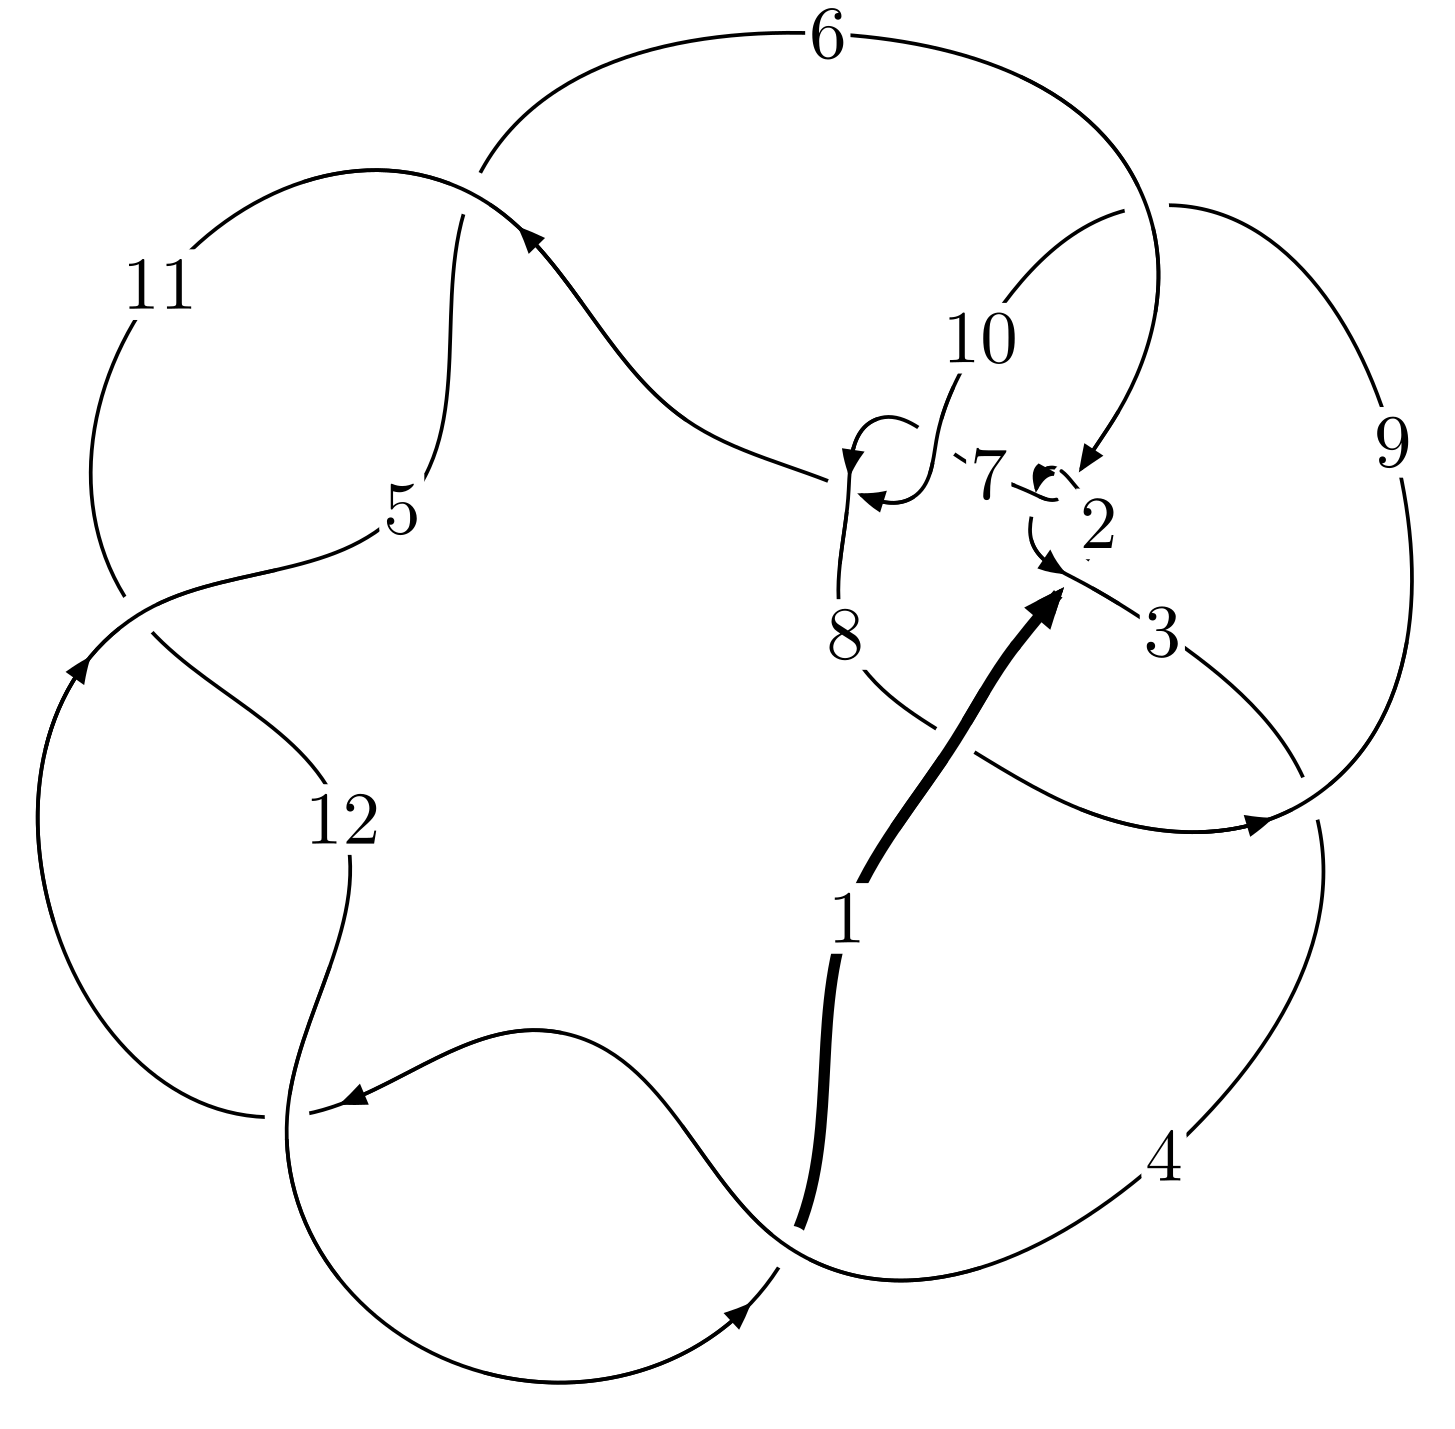
\includegraphics[width=112pt]{../../../GIT/diagram.site/Diagrams/png/1414_12a_0613.png}\\
\ \ \ A knot diagram\footnotemark}&
\allowdisplaybreaks
\textbf{Linearized knot diagam} \\
\cline{2-2}
 &
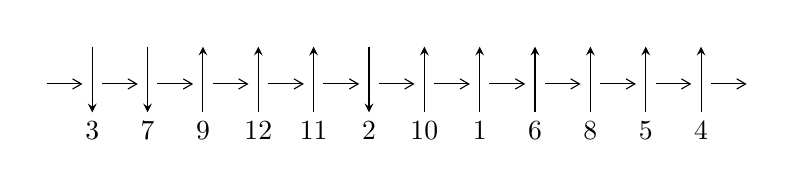
\begin{tikzpicture}[x=20pt, y=17pt]
	% nodes
	\node (C0) at (0, 0) {};
	\node (C1) at (1, 0) {};
	\node (C1U) at (1, +1) {};
	\node (C1D) at (1, -1) {3};

	\node (C2) at (2, 0) {};
	\node (C2U) at (2, +1) {};
	\node (C2D) at (2, -1) {7};

	\node (C3) at (3, 0) {};
	\node (C3U) at (3, +1) {};
	\node (C3D) at (3, -1) {9};

	\node (C4) at (4, 0) {};
	\node (C4U) at (4, +1) {};
	\node (C4D) at (4, -1) {12};

	\node (C5) at (5, 0) {};
	\node (C5U) at (5, +1) {};
	\node (C5D) at (5, -1) {11};

	\node (C6) at (6, 0) {};
	\node (C6U) at (6, +1) {};
	\node (C6D) at (6, -1) {2};

	\node (C7) at (7, 0) {};
	\node (C7U) at (7, +1) {};
	\node (C7D) at (7, -1) {10};

	\node (C8) at (8, 0) {};
	\node (C8U) at (8, +1) {};
	\node (C8D) at (8, -1) {1};

	\node (C9) at (9, 0) {};
	\node (C9U) at (9, +1) {};
	\node (C9D) at (9, -1) {6};

	\node (C10) at (10, 0) {};
	\node (C10U) at (10, +1) {};
	\node (C10D) at (10, -1) {8};

	\node (C11) at (11, 0) {};
	\node (C11U) at (11, +1) {};
	\node (C11D) at (11, -1) {5};

	\node (C12) at (12, 0) {};
	\node (C12U) at (12, +1) {};
	\node (C12D) at (12, -1) {4};
	\node (C13) at (13, 0) {};

	% arrows
	\draw[->,>={angle 60}]
	(C0) edge (C1) (C1) edge (C2) (C2) edge (C3) (C3) edge (C4) (C4) edge (C5) (C5) edge (C6) (C6) edge (C7) (C7) edge (C8) (C8) edge (C9) (C9) edge (C10) (C10) edge (C11) (C11) edge (C12) (C12) edge (C13) ;	\draw[->,>=stealth]
	(C1U) edge (C1D) (C2U) edge (C2D) (C3D) edge (C3U) (C4D) edge (C4U) (C5D) edge (C5U) (C6U) edge (C6D) (C7D) edge (C7U) (C8D) edge (C8U) (C9D) edge (C9U) (C10D) edge (C10U) (C11D) edge (C11U) (C12D) edge (C12U) ;
	\end{tikzpicture} \\
\hhline{~~} \\& 
\textbf{Solving Sequence} \\ \cline{2-2} 
 &
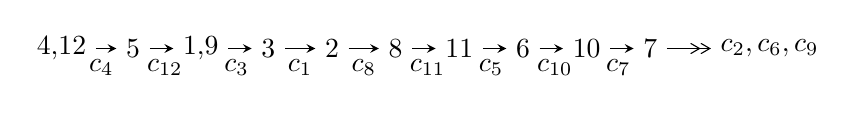
\begin{tikzpicture}[x=23pt, y=7pt]
	% node
	\node (A0) at (-1/8, 0) {4,12};
	\node (A1) at (1, 0) {5};
	\node (A2) at (33/16, 0) {1,9};
	\node (A3) at (25/8, 0) {3};
	\node (A4) at (33/8, 0) {2};
	\node (A5) at (41/8, 0) {8};
	\node (A6) at (49/8, 0) {11};
	\node (A7) at (57/8, 0) {6};
	\node (A8) at (65/8, 0) {10};
	\node (A9) at (73/8, 0) {7};
	\node (C1) at (1/2, -1) {$c_{4}$};
	\node (C2) at (3/2, -1) {$c_{12}$};
	\node (C3) at (21/8, -1) {$c_{3}$};
	\node (C4) at (29/8, -1) {$c_{1}$};
	\node (C5) at (37/8, -1) {$c_{8}$};
	\node (C6) at (45/8, -1) {$c_{11}$};
	\node (C7) at (53/8, -1) {$c_{5}$};
	\node (C8) at (61/8, -1) {$c_{10}$};
	\node (C9) at (69/8, -1) {$c_{7}$};
	\node (A10) at (11, 0) {$c_{2},c_{6},c_{9}$};

	% edge
	\draw[->,>=stealth]	
	(A0) edge (A1) (A1) edge (A2) (A2) edge (A3) (A3) edge (A4) (A4) edge (A5) (A5) edge (A6) (A6) edge (A7) (A7) edge (A8) (A8) edge (A9) ;
	\draw[->>,>={angle 60}]	
	(A9) edge (A10);
\end{tikzpicture} \\ 

\end{tabular} \\

\footnotetext{
The image of knot diagram is generated by the software ``\textbf{Draw programme}" developed by Andrew Bartholomew(\url{http://www.layer8.co.uk/maths/draw/index.htm\#Running-draw}), where we modified some parts for our purpose(\url{https://github.com/CATsTAILs/LinksPainter}).
}\phantom \\ \newline 
\centering \textbf{Ideals for irreducible components\footnotemark of $X_{\text{par}}$} 
 
\begin{align*}
I^u_{1}&=\langle 
-2.03882\times10^{79} u^{78}+2.23239\times10^{79} u^{77}+\cdots+2.55472\times10^{80} b-1.96227\times10^{79},\\
\phantom{I^u_{1}}&\phantom{= \langle  }-8.18368\times10^{80} u^{78}+6.97572\times10^{80} u^{77}+\cdots+1.02189\times10^{81} a-2.19255\times10^{81},\;u^{79}-2 u^{78}+\cdots- u^2+1\rangle \\
I^u_{2}&=\langle 
b,\;2 a-1,\;u^2- u+1\rangle \\
\\
\end{align*}
\raggedright * 2 irreducible components of $\dim_{\mathbb{C}}=0$, with total 81 representations.\\
\footnotetext{All coefficients of polynomials are rational numbers. But the coefficients are sometimes approximated in decimal forms when there is not enough margin.}
\newpage
\renewcommand{\arraystretch}{1}
\centering \section*{I. $I^u_{1}= \langle -2.04\times10^{79} u^{78}+2.23\times10^{79} u^{77}+\cdots+2.55\times10^{80} b-1.96\times10^{79},\;-8.18\times10^{80} u^{78}+6.98\times10^{80} u^{77}+\cdots+1.02\times10^{81} a-2.19\times10^{81},\;u^{79}-2 u^{78}+\cdots- u^2+1 \rangle$}
\flushleft \textbf{(i) Arc colorings}\\
\begin{tabular}{m{7pt} m{180pt} m{7pt} m{180pt} }
\flushright $a_{4}=$&$\begin{pmatrix}1\\0\end{pmatrix}$ \\
\flushright $a_{12}=$&$\begin{pmatrix}0\\u\end{pmatrix}$ \\
\flushright $a_{5}=$&$\begin{pmatrix}1\\- u^2\end{pmatrix}$ \\
\flushright $a_{1}=$&$\begin{pmatrix}u\\u\end{pmatrix}$ \\
\flushright $a_{9}=$&$\begin{pmatrix}0.800839 u^{78}-0.682630 u^{77}+\cdots+3.30143 u+2.14559\\0.0798060 u^{78}-0.0873829 u^{77}+\cdots+1.62926 u+0.0768097\end{pmatrix}$ \\
\flushright $a_{3}=$&$\begin{pmatrix}0.00402796 u^{78}-0.254054 u^{77}+\cdots-0.699999 u-0.768387\\0.181867 u^{78}-0.302615 u^{77}+\cdots-0.399516 u-0.657378\end{pmatrix}$ \\
\flushright $a_{2}=$&$\begin{pmatrix}0.867844 u^{78}-1.44502 u^{77}+\cdots-1.58649 u-0.804996\\0.630533 u^{78}-0.911235 u^{77}+\cdots+1.37596 u-0.234189\end{pmatrix}$ \\
\flushright $a_{8}=$&$\begin{pmatrix}0.747578 u^{78}-1.04412 u^{77}+\cdots+2.58040 u+1.29877\\0.0265456 u^{78}-0.448872 u^{77}+\cdots+0.908223 u-0.770009\end{pmatrix}$ \\
\flushright $a_{11}=$&$\begin{pmatrix}- u\\u^3+u\end{pmatrix}$ \\
\flushright $a_{6}=$&$\begin{pmatrix}u^2+1\\- u^4-2 u^2\end{pmatrix}$ \\
\flushright $a_{10}=$&$\begin{pmatrix}0.885426 u^{78}-1.25091 u^{77}+\cdots+3.14176 u+1.13115\\0.101593 u^{78}-0.552926 u^{77}+\cdots+1.81848 u-0.679272\end{pmatrix}$ \\
\flushright $a_{7}=$&$\begin{pmatrix}-0.411380 u^{78}+0.671759 u^{77}+\cdots-1.60537 u+0.403544\\-0.193891 u^{78}+0.272615 u^{77}+\cdots-1.17977 u-0.155029\end{pmatrix}$\\&\end{tabular}
\flushleft \textbf{(ii) Obstruction class $= -1$}\\~\\
\flushleft \textbf{(iii) Cusp Shapes $= -1.00132 u^{78}-2.47157 u^{77}+\cdots-17.5561 u-2.90148$}\\~\\
\newpage\renewcommand{\arraystretch}{1}
\flushleft \textbf{(iv) u-Polynomials at the component}\newline \\
\begin{tabular}{m{50pt}|m{274pt}}
Crossings & \hspace{64pt}u-Polynomials at each crossing \\
\hline $$\begin{aligned}c_{1}\end{aligned}$$&$\begin{aligned}
&u^{79}+28 u^{78}+\cdots+2 u+1
\end{aligned}$\\
\hline $$\begin{aligned}c_{2},c_{6}\end{aligned}$$&$\begin{aligned}
&u^{79}-2 u^{78}+\cdots+4 u-1
\end{aligned}$\\
\hline $$\begin{aligned}c_{3}\end{aligned}$$&$\begin{aligned}
&u^{79}- u^{78}+\cdots+224 u-64
\end{aligned}$\\
\hline $$\begin{aligned}c_{4},c_{5},c_{11}\\c_{12}\end{aligned}$$&$\begin{aligned}
&u^{79}+2 u^{78}+\cdots+u^2-1
\end{aligned}$\\
\hline $$\begin{aligned}c_{7},c_{10}\end{aligned}$$&$\begin{aligned}
&u^{79}+3 u^{78}+\cdots+8 u-16
\end{aligned}$\\
\hline $$\begin{aligned}c_{8}\end{aligned}$$&$\begin{aligned}
&4(4 u^{79}+62 u^{78}+\cdots-19 u-983)
\end{aligned}$\\
\hline $$\begin{aligned}c_{9}\end{aligned}$$&$\begin{aligned}
&4(4 u^{79}+70 u^{78}+\cdots+5805 u-1399)
\end{aligned}$\\
\hline
\end{tabular}\\~\\
\newpage\renewcommand{\arraystretch}{1}
\flushleft \textbf{(v) Riley Polynomials at the component}\newline \\
\begin{tabular}{m{50pt}|m{274pt}}
Crossings & \hspace{64pt}Riley Polynomials at each crossing \\
\hline $$\begin{aligned}c_{1}\end{aligned}$$&$\begin{aligned}
&y^{79}+40 y^{78}+\cdots-82 y-1
\end{aligned}$\\
\hline $$\begin{aligned}c_{2},c_{6}\end{aligned}$$&$\begin{aligned}
&y^{79}-28 y^{78}+\cdots+2 y-1
\end{aligned}$\\
\hline $$\begin{aligned}c_{3}\end{aligned}$$&$\begin{aligned}
&y^{79}+15 y^{78}+\cdots-1536 y-4096
\end{aligned}$\\
\hline $$\begin{aligned}c_{4},c_{5},c_{11}\\c_{12}\end{aligned}$$&$\begin{aligned}
&y^{79}+92 y^{78}+\cdots+2 y-1
\end{aligned}$\\
\hline $$\begin{aligned}c_{7},c_{10}\end{aligned}$$&$\begin{aligned}
&y^{79}-47 y^{78}+\cdots+10272 y-256
\end{aligned}$\\
\hline $$\begin{aligned}c_{8}\end{aligned}$$&$\begin{aligned}
&16(16 y^{79}+916 y^{78}+\cdots-1527221 y-966289)
\end{aligned}$\\
\hline $$\begin{aligned}c_{9}\end{aligned}$$&$\begin{aligned}
&16(16 y^{79}-828 y^{78}+\cdots+2.53292\times10^{7} y-1957201)
\end{aligned}$\\
\hline
\end{tabular}\\~\\
\newpage\flushleft \textbf{(vi) Complex Volumes and Cusp Shapes}
$$\begin{array}{c|c|c}  
\text{Solutions to }I^u_{1}& \I (\text{vol} + \sqrt{-1}CS) & \text{Cusp shape}\\
 \hline 
\begin{aligned}
u &= \phantom{-}0.562843 + 0.832702 I \\
a &= -0.56281 + 1.45509 I \\
b &= \phantom{-}0.98702 + 1.13654 I\end{aligned}
 & \phantom{-}1.52292 + 13.66740 I & \phantom{-0.000000 } 0 \\ \hline\begin{aligned}
u &= \phantom{-}0.562843 - 0.832702 I \\
a &= -0.56281 - 1.45509 I \\
b &= \phantom{-}0.98702 - 1.13654 I\end{aligned}
 & \phantom{-}1.52292 - 13.66740 I & \phantom{-0.000000 } 0 \\ \hline\begin{aligned}
u &= -0.741395 + 0.678986 I \\
a &= \phantom{-}0.310828 + 0.208855 I \\
b &= -0.225354 + 0.507570 I\end{aligned}
 & \phantom{-}1.56279 - 2.63526 I & \phantom{-0.000000 } 0 \\ \hline\begin{aligned}
u &= -0.741395 - 0.678986 I \\
a &= \phantom{-}0.310828 - 0.208855 I \\
b &= -0.225354 - 0.507570 I\end{aligned}
 & \phantom{-}1.56279 + 2.63526 I & \phantom{-0.000000 } 0 \\ \hline\begin{aligned}
u &= -0.579273 + 0.830831 I \\
a &= \phantom{-}0.417162 + 1.259300 I \\
b &= -0.933225 + 0.954782 I\end{aligned}
 & \phantom{-}3.15768 - 7.68910 I & \phantom{-0.000000 } 0 \\ \hline\begin{aligned}
u &= -0.579273 - 0.830831 I \\
a &= \phantom{-}0.417162 - 1.259300 I \\
b &= -0.933225 - 0.954782 I\end{aligned}
 & \phantom{-}3.15768 + 7.68910 I & \phantom{-0.000000 } 0 \\ \hline\begin{aligned}
u &= \phantom{-}0.568605 + 0.766638 I \\
a &= -0.846313 + 0.755150 I \\
b &= \phantom{-}0.443486 + 1.011560 I\end{aligned}
 & -3.94285 + 6.03723 I & \phantom{-0.000000 } 0 \\ \hline\begin{aligned}
u &= \phantom{-}0.568605 - 0.766638 I \\
a &= -0.846313 - 0.755150 I \\
b &= \phantom{-}0.443486 - 1.011560 I\end{aligned}
 & -3.94285 - 6.03723 I & \phantom{-0.000000 } 0 \\ \hline\begin{aligned}
u &= \phantom{-}0.338960 + 0.869847 I \\
a &= \phantom{-}0.612024 - 1.143240 I \\
b &= -0.336341 - 1.122390 I\end{aligned}
 & -5.58907 + 1.26010 I & \phantom{-0.000000 } 0 \\ \hline\begin{aligned}
u &= \phantom{-}0.338960 - 0.869847 I \\
a &= \phantom{-}0.612024 + 1.143240 I \\
b &= -0.336341 + 1.122390 I\end{aligned}
 & -5.58907 - 1.26010 I & \phantom{-0.000000 } 0\\
 \hline 
 \end{array}$$\newpage$$\begin{array}{c|c|c}  
\text{Solutions to }I^u_{1}& \I (\text{vol} + \sqrt{-1}CS) & \text{Cusp shape}\\
 \hline 
\begin{aligned}
u &= \phantom{-}0.370841 + 0.777492 I \\
a &= \phantom{-}0.33367 - 1.64645 I \\
b &= -1.06752 - 1.25567 I\end{aligned}
 & -2.35487 + 7.66759 I & \phantom{-0.000000 } 0 \\ \hline\begin{aligned}
u &= \phantom{-}0.370841 - 0.777492 I \\
a &= \phantom{-}0.33367 + 1.64645 I \\
b &= -1.06752 + 1.25567 I\end{aligned}
 & -2.35487 - 7.66759 I & \phantom{-0.000000 } 0 \\ \hline\begin{aligned}
u &= \phantom{-}0.501863 + 1.023240 I \\
a &= \phantom{-}0.790922 - 0.128653 I \\
b &= \phantom{-}0.562719 - 0.703503 I\end{aligned}
 & \phantom{-}0.48015 - 4.91507 I & \phantom{-0.000000 } 0 \\ \hline\begin{aligned}
u &= \phantom{-}0.501863 - 1.023240 I \\
a &= \phantom{-}0.790922 + 0.128653 I \\
b &= \phantom{-}0.562719 + 0.703503 I\end{aligned}
 & \phantom{-}0.48015 + 4.91507 I & \phantom{-0.000000 } 0 \\ \hline\begin{aligned}
u &= -0.331748 + 0.759592 I \\
a &= -0.17186 - 1.41166 I \\
b &= \phantom{-}1.020660 - 0.871256 I\end{aligned}
 & -0.93419 - 2.69523 I & \phantom{-0.000000 } 0 \\ \hline\begin{aligned}
u &= -0.331748 - 0.759592 I \\
a &= -0.17186 + 1.41166 I \\
b &= \phantom{-}1.020660 + 0.871256 I\end{aligned}
 & -0.93419 + 2.69523 I & \phantom{-0.000000 } 0 \\ \hline\begin{aligned}
u &= -0.801592 + 0.090466 I \\
a &= -0.152170 - 0.181666 I \\
b &= \phantom{-}0.785054 + 0.668987 I\end{aligned}
 & \phantom{-}5.40107 + 3.12470 I & \phantom{-}10.83520 - 3.71526 I \\ \hline\begin{aligned}
u &= -0.801592 - 0.090466 I \\
a &= -0.152170 + 0.181666 I \\
b &= \phantom{-}0.785054 - 0.668987 I\end{aligned}
 & \phantom{-}5.40107 - 3.12470 I & \phantom{-}10.83520 + 3.71526 I \\ \hline\begin{aligned}
u &= \phantom{-}0.771291 + 0.077638 I \\
a &= \phantom{-}0.207850 - 0.230451 I \\
b &= -0.869715 + 0.901562 I\end{aligned}
 & \phantom{-}3.80470 - 9.23717 I & \phantom{-}8.33412 + 6.93035 I \\ \hline\begin{aligned}
u &= \phantom{-}0.771291 - 0.077638 I \\
a &= \phantom{-}0.207850 + 0.230451 I \\
b &= -0.869715 - 0.901562 I\end{aligned}
 & \phantom{-}3.80470 + 9.23717 I & \phantom{-}8.33412 - 6.93035 I\\
 \hline 
 \end{array}$$\newpage$$\begin{array}{c|c|c}  
\text{Solutions to }I^u_{1}& \I (\text{vol} + \sqrt{-1}CS) & \text{Cusp shape}\\
 \hline 
\begin{aligned}
u &= -0.553421 + 1.128580 I \\
a &= -0.458687 - 0.080550 I \\
b &= -0.373011 - 0.438940 I\end{aligned}
 & \phantom{-}1.82683 - 1.50251 I & \phantom{-0.000000 } 0 \\ \hline\begin{aligned}
u &= -0.553421 - 1.128580 I \\
a &= -0.458687 + 0.080550 I \\
b &= -0.373011 + 0.438940 I\end{aligned}
 & \phantom{-}1.82683 + 1.50251 I & \phantom{-0.000000 } 0 \\ \hline\begin{aligned}
u &= -0.231967 + 0.666632 I \\
a &= -0.366445 - 0.960576 I \\
b &= \phantom{-}0.783116 - 0.050253 I\end{aligned}
 & -0.79258 - 1.89815 I & \phantom{-}1.36018 + 5.78831 I \\ \hline\begin{aligned}
u &= -0.231967 - 0.666632 I \\
a &= -0.366445 + 0.960576 I \\
b &= \phantom{-}0.783116 + 0.050253 I\end{aligned}
 & -0.79258 + 1.89815 I & \phantom{-}1.36018 - 5.78831 I \\ \hline\begin{aligned}
u &= -0.182894 + 0.674305 I \\
a &= -0.009457 - 1.377310 I \\
b &= \phantom{-}0.480502 - 0.004250 I\end{aligned}
 & -0.67916 - 1.82123 I & \phantom{-}2.42742 + 5.42469 I \\ \hline\begin{aligned}
u &= -0.182894 - 0.674305 I \\
a &= -0.009457 + 1.377310 I \\
b &= \phantom{-}0.480502 + 0.004250 I\end{aligned}
 & -0.67916 + 1.82123 I & \phantom{-}2.42742 - 5.42469 I \\ \hline\begin{aligned}
u &= \phantom{-}0.391868 + 0.577092 I \\
a &= -0.872126 - 0.595448 I \\
b &= -0.209144 + 0.629764 I\end{aligned}
 & -1.69314 - 1.96298 I & -0.140339 - 0.849160 I \\ \hline\begin{aligned}
u &= \phantom{-}0.391868 - 0.577092 I \\
a &= -0.872126 + 0.595448 I \\
b &= -0.209144 - 0.629764 I\end{aligned}
 & -1.69314 + 1.96298 I & -0.140339 + 0.849160 I \\ \hline\begin{aligned}
u &= \phantom{-}0.654803 + 0.208319 I \\
a &= -0.109482 - 0.416917 I \\
b &= -0.076780 + 0.829628 I\end{aligned}
 & -2.27524 - 1.80401 I & \phantom{-}0.55826 + 3.15083 I \\ \hline\begin{aligned}
u &= \phantom{-}0.654803 - 0.208319 I \\
a &= -0.109482 + 0.416917 I \\
b &= -0.076780 - 0.829628 I\end{aligned}
 & -2.27524 + 1.80401 I & \phantom{-}0.55826 - 3.15083 I\\
 \hline 
 \end{array}$$\newpage$$\begin{array}{c|c|c}  
\text{Solutions to }I^u_{1}& \I (\text{vol} + \sqrt{-1}CS) & \text{Cusp shape}\\
 \hline 
\begin{aligned}
u &= -0.049356 + 0.679141 I \\
a &= -4.06707 - 7.37445 I \\
b &= \phantom{-}0.211661 - 0.213403 I\end{aligned}
 & \phantom{-}0.65806 + 2.13491 I & -3.7911 + 41.5128 I \\ \hline\begin{aligned}
u &= -0.049356 - 0.679141 I \\
a &= -4.06707 + 7.37445 I \\
b &= \phantom{-}0.211661 + 0.213403 I\end{aligned}
 & \phantom{-}0.65806 - 2.13491 I & -3.7911 - 41.5128 I \\ \hline\begin{aligned}
u &= -0.345401 + 0.562828 I \\
a &= \phantom{-}1.079840 - 0.026704 I \\
b &= \phantom{-}1.43886 + 0.80805 I\end{aligned}
 & \phantom{-}2.60435 - 5.50536 I & \phantom{-}8.17810 + 10.12100 I \\ \hline\begin{aligned}
u &= -0.345401 - 0.562828 I \\
a &= \phantom{-}1.079840 + 0.026704 I \\
b &= \phantom{-}1.43886 - 0.80805 I\end{aligned}
 & \phantom{-}2.60435 + 5.50536 I & \phantom{-}8.17810 - 10.12100 I \\ \hline\begin{aligned}
u &= \phantom{-}0.331681 + 0.523775 I \\
a &= -1.065230 + 0.540959 I \\
b &= -1.11153 + 1.03548 I\end{aligned}
 & \phantom{-}3.09371 + 0.52538 I & \phantom{-}9.90827 - 3.67207 I \\ \hline\begin{aligned}
u &= \phantom{-}0.331681 - 0.523775 I \\
a &= -1.065230 - 0.540959 I \\
b &= -1.11153 - 1.03548 I\end{aligned}
 & \phantom{-}3.09371 - 0.52538 I & \phantom{-}9.90827 + 3.67207 I \\ \hline\begin{aligned}
u &= \phantom{-}0.170277 + 0.493014 I \\
a &= \phantom{-}0.73593 + 1.99770 I \\
b &= -0.348401 + 0.520479 I\end{aligned}
 & \phantom{-}1.35750 + 0.77449 I & \phantom{-}3.79816 + 1.46964 I \\ \hline\begin{aligned}
u &= \phantom{-}0.170277 - 0.493014 I \\
a &= \phantom{-}0.73593 - 1.99770 I \\
b &= -0.348401 - 0.520479 I\end{aligned}
 & \phantom{-}1.35750 - 0.77449 I & \phantom{-}3.79816 - 1.46964 I \\ \hline\begin{aligned}
u &= \phantom{-}0.485463 + 0.020121 I \\
a &= -0.398789 - 1.077720 I \\
b &= \phantom{-}0.850535 + 0.743850 I\end{aligned}
 & -0.04571 + 4.74027 I & \phantom{-}6.49908 - 5.57095 I \\ \hline\begin{aligned}
u &= \phantom{-}0.485463 - 0.020121 I \\
a &= -0.398789 + 1.077720 I \\
b &= \phantom{-}0.850535 - 0.743850 I\end{aligned}
 & -0.04571 - 4.74027 I & \phantom{-}6.49908 + 5.57095 I\\
 \hline 
 \end{array}$$\newpage$$\begin{array}{c|c|c}  
\text{Solutions to }I^u_{1}& \I (\text{vol} + \sqrt{-1}CS) & \text{Cusp shape}\\
 \hline 
\begin{aligned}
u &= \phantom{-}0.334435 + 0.319559 I \\
a &= -1.47425 + 2.33133 I \\
b &= \phantom{-}0.404340 + 1.278840 I\end{aligned}
 & \phantom{-}3.64262 + 2.01368 I & \phantom{-}11.35214 - 6.18075 I \\ \hline\begin{aligned}
u &= \phantom{-}0.334435 - 0.319559 I \\
a &= -1.47425 - 2.33133 I \\
b &= \phantom{-}0.404340 - 1.278840 I\end{aligned}
 & \phantom{-}3.64262 - 2.01368 I & \phantom{-}11.35214 + 6.18075 I \\ \hline\begin{aligned}
u &= \phantom{-}0.00649 + 1.54238 I \\
a &= \phantom{-}0.21865 - 2.91487 I \\
b &= \phantom{-}0.21929 - 2.08709 I\end{aligned}
 & -2.64074 + 2.57318 I & \phantom{-0.000000 } 0 \\ \hline\begin{aligned}
u &= \phantom{-}0.00649 - 1.54238 I \\
a &= \phantom{-}0.21865 + 2.91487 I \\
b &= \phantom{-}0.21929 + 2.08709 I\end{aligned}
 & -2.64074 - 2.57318 I & \phantom{-0.000000 } 0 \\ \hline\begin{aligned}
u &= -0.351711 + 0.263028 I \\
a &= \phantom{-}1.52295 + 2.40752 I \\
b &= -0.773586 + 1.088950 I\end{aligned}
 & \phantom{-}3.41440 + 2.89559 I & \phantom{-}11.29503 - 0.80048 I \\ \hline\begin{aligned}
u &= -0.351711 - 0.263028 I \\
a &= \phantom{-}1.52295 - 2.40752 I \\
b &= -0.773586 - 1.088950 I\end{aligned}
 & \phantom{-}3.41440 - 2.89559 I & \phantom{-}11.29503 + 0.80048 I \\ \hline\begin{aligned}
u &= \phantom{-}0.05749 + 1.56794 I \\
a &= \phantom{-}1.60542 - 1.04355 I \\
b &= \phantom{-}1.76518 - 0.94006 I\end{aligned}
 & -4.04246 + 1.74152 I & \phantom{-0.000000 } 0 \\ \hline\begin{aligned}
u &= \phantom{-}0.05749 - 1.56794 I \\
a &= \phantom{-}1.60542 + 1.04355 I \\
b &= \phantom{-}1.76518 + 0.94006 I\end{aligned}
 & -4.04246 - 1.74152 I & \phantom{-0.000000 } 0 \\ \hline\begin{aligned}
u &= -0.06787 + 1.57326 I \\
a &= -1.88218 - 0.50014 I \\
b &= -2.03284 - 0.61356 I\end{aligned}
 & -4.67331 - 6.86430 I & \phantom{-0.000000 } 0 \\ \hline\begin{aligned}
u &= -0.06787 - 1.57326 I \\
a &= -1.88218 + 0.50014 I \\
b &= -2.03284 + 0.61356 I\end{aligned}
 & -4.67331 + 6.86430 I & \phantom{-0.000000 } 0\\
 \hline 
 \end{array}$$\newpage$$\begin{array}{c|c|c}  
\text{Solutions to }I^u_{1}& \I (\text{vol} + \sqrt{-1}CS) & \text{Cusp shape}\\
 \hline 
\begin{aligned}
u &= \phantom{-}0.02636 + 1.58296 I \\
a &= -0.03578 - 1.50159 I \\
b &= \phantom{-}0.705909 - 0.781446 I\end{aligned}
 & -5.92590 + 1.33377 I & \phantom{-0.000000 } 0 \\ \hline\begin{aligned}
u &= \phantom{-}0.02636 - 1.58296 I \\
a &= -0.03578 + 1.50159 I \\
b &= \phantom{-}0.705909 + 0.781446 I\end{aligned}
 & -5.92590 - 1.33377 I & \phantom{-0.000000 } 0 \\ \hline\begin{aligned}
u &= \phantom{-}0.18347 + 1.58484 I \\
a &= \phantom{-}0.360763 - 0.757569 I \\
b &= -0.261769 - 0.839182 I\end{aligned}
 & -8.84874 + 0.48741 I & \phantom{-0.000000 } 0 \\ \hline\begin{aligned}
u &= \phantom{-}0.18347 - 1.58484 I \\
a &= \phantom{-}0.360763 + 0.757569 I \\
b &= -0.261769 + 0.839182 I\end{aligned}
 & -8.84874 - 0.48741 I & \phantom{-0.000000 } 0 \\ \hline\begin{aligned}
u &= -0.398279 + 0.013530 I \\
a &= \phantom{-}0.938259 + 1.052560 I \\
b &= -0.839928 - 0.266112 I\end{aligned}
 & \phantom{-}1.200820 + 0.135633 I & \phantom{-}10.41521 - 0.49094 I \\ \hline\begin{aligned}
u &= -0.398279 - 0.013530 I \\
a &= \phantom{-}0.938259 - 1.052560 I \\
b &= -0.839928 + 0.266112 I\end{aligned}
 & \phantom{-}1.200820 - 0.135633 I & \phantom{-}10.41521 + 0.49094 I \\ \hline\begin{aligned}
u &= -0.04900 + 1.60834 I \\
a &= -0.163063 + 0.427641 I \\
b &= -0.996770 + 0.017416 I\end{aligned}
 & -8.65958 - 2.85508 I & \phantom{-0.000000 } 0 \\ \hline\begin{aligned}
u &= -0.04900 - 1.60834 I \\
a &= -0.163063 - 0.427641 I \\
b &= -0.996770 - 0.017416 I\end{aligned}
 & -8.65958 + 2.85508 I & \phantom{-0.000000 } 0 \\ \hline\begin{aligned}
u &= -0.01243 + 1.61005 I \\
a &= \phantom{-}4.20907 - 1.82134 I \\
b &= -0.282683 - 0.182370 I\end{aligned}
 & -7.26471 + 1.91119 I & \phantom{-0.000000 } 0 \\ \hline\begin{aligned}
u &= -0.01243 - 1.61005 I \\
a &= \phantom{-}4.20907 + 1.82134 I \\
b &= -0.282683 + 0.182370 I\end{aligned}
 & -7.26471 - 1.91119 I & \phantom{-0.000000 } 0\\
 \hline 
 \end{array}$$\newpage$$\begin{array}{c|c|c}  
\text{Solutions to }I^u_{1}& \I (\text{vol} + \sqrt{-1}CS) & \text{Cusp shape}\\
 \hline 
\begin{aligned}
u &= -0.09234 + 1.63211 I \\
a &= -0.52019 + 1.88202 I \\
b &= -1.13740 + 1.31093 I\end{aligned}
 & -9.19819 - 4.29526 I & \phantom{-0.000000 } 0 \\ \hline\begin{aligned}
u &= -0.09234 - 1.63211 I \\
a &= -0.52019 - 1.88202 I \\
b &= -1.13740 - 1.31093 I\end{aligned}
 & -9.19819 + 4.29526 I & \phantom{-0.000000 } 0 \\ \hline\begin{aligned}
u &= \phantom{-}0.10241 + 1.63406 I \\
a &= \phantom{-}0.44688 + 2.25253 I \\
b &= \phantom{-}1.13698 + 1.65533 I\end{aligned}
 & -10.6594 + 9.4536 I & \phantom{-0.000000 } 0 \\ \hline\begin{aligned}
u &= \phantom{-}0.10241 - 1.63406 I \\
a &= \phantom{-}0.44688 - 2.25253 I \\
b &= \phantom{-}1.13698 - 1.65533 I\end{aligned}
 & -10.6594 - 9.4536 I & \phantom{-0.000000 } 0 \\ \hline\begin{aligned}
u &= -0.19581 + 1.62772 I \\
a &= -0.028644 - 1.044970 I \\
b &= \phantom{-}0.575863 - 0.832632 I\end{aligned}
 & -6.29500 - 6.01229 I & \phantom{-0.000000 } 0 \\ \hline\begin{aligned}
u &= -0.19581 - 1.62772 I \\
a &= -0.028644 + 1.044970 I \\
b &= \phantom{-}0.575863 + 0.832632 I\end{aligned}
 & -6.29500 + 6.01229 I & \phantom{-0.000000 } 0 \\ \hline\begin{aligned}
u &= \phantom{-}0.16718 + 1.63714 I \\
a &= \phantom{-}0.27278 - 1.56528 I \\
b &= -0.651768 - 1.223680 I\end{aligned}
 & -12.1301 + 8.8302 I & \phantom{-0.000000 } 0 \\ \hline\begin{aligned}
u &= \phantom{-}0.16718 - 1.63714 I \\
a &= \phantom{-}0.27278 + 1.56528 I \\
b &= -0.651768 + 1.223680 I\end{aligned}
 & -12.1301 - 8.8302 I & \phantom{-0.000000 } 0 \\ \hline\begin{aligned}
u &= -0.04375 + 1.64757 I \\
a &= -0.028083 + 1.158780 I \\
b &= -0.425950 + 0.521893 I\end{aligned}
 & -8.90382 - 2.51455 I & \phantom{-0.000000 } 0 \\ \hline\begin{aligned}
u &= -0.04375 - 1.64757 I \\
a &= -0.028083 - 1.158780 I \\
b &= -0.425950 - 0.521893 I\end{aligned}
 & -8.90382 + 2.51455 I & \phantom{-0.000000 } 0\\
 \hline 
 \end{array}$$\newpage$$\begin{array}{c|c|c}  
\text{Solutions to }I^u_{1}& \I (\text{vol} + \sqrt{-1}CS) & \text{Cusp shape}\\
 \hline 
\begin{aligned}
u &= \phantom{-}0.09434 + 1.65580 I \\
a &= -0.15890 + 1.82134 I \\
b &= \phantom{-}0.48529 + 1.40625 I\end{aligned}
 & -14.3142 + 2.9381 I & \phantom{-0.000000 } 0 \\ \hline\begin{aligned}
u &= \phantom{-}0.09434 - 1.65580 I \\
a &= -0.15890 - 1.82134 I \\
b &= \phantom{-}0.48529 - 1.40625 I\end{aligned}
 & -14.3142 - 2.9381 I & \phantom{-0.000000 } 0 \\ \hline\begin{aligned}
u &= -0.17049 + 1.65268 I \\
a &= \phantom{-}0.18613 - 1.81679 I \\
b &= \phantom{-}1.00691 - 1.19883 I\end{aligned}
 & -5.29842 - 10.57260 I & \phantom{-0.000000 } 0 \\ \hline\begin{aligned}
u &= -0.17049 - 1.65268 I \\
a &= \phantom{-}0.18613 + 1.81679 I \\
b &= \phantom{-}1.00691 + 1.19883 I\end{aligned}
 & -5.29842 + 10.57260 I & \phantom{-0.000000 } 0 \\ \hline\begin{aligned}
u &= \phantom{-}0.16564 + 1.65397 I \\
a &= -0.12615 - 2.02494 I \\
b &= -1.04487 - 1.34226 I\end{aligned}
 & -6.9597 + 16.4745 I & \phantom{-0.000000 } 0 \\ \hline\begin{aligned}
u &= \phantom{-}0.16564 - 1.65397 I \\
a &= -0.12615 + 2.02494 I \\
b &= -1.04487 + 1.34226 I\end{aligned}
 & -6.9597 - 16.4745 I & \phantom{-0.000000 } 0 \\ \hline\begin{aligned}
u &= -0.295195\phantom{ +0.000000I} \\
a &= \phantom{-}2.10631\phantom{ +0.000000I} \\
b &= -0.614585\phantom{ +0.000000I}\end{aligned}
 & \phantom{-}0.931731\phantom{ +0.000000I} & \phantom{-}11.9810\phantom{ +0.000000I} \\ \hline\begin{aligned}
u &= \phantom{-}0.06001 + 1.71584 I \\
a &= -0.304602 + 0.966268 I \\
b &= -0.057490 + 0.749405 I\end{aligned}
 & -9.46041 - 2.81380 I & \phantom{-0.000000 } 0 \\ \hline\begin{aligned}
u &= \phantom{-}0.06001 - 1.71584 I \\
a &= -0.304602 - 0.966268 I \\
b &= -0.057490 - 0.749405 I\end{aligned}
 & -9.46041 + 2.81380 I & \phantom{-0.000000 } 0\\
 \hline 
 \end{array}$$\newpage\newpage\renewcommand{\arraystretch}{1}
\centering \section*{II. $I^u_{2}= \langle b,\;2 a-1,\;u^2- u+1 \rangle$}
\flushleft \textbf{(i) Arc colorings}\\
\begin{tabular}{m{7pt} m{180pt} m{7pt} m{180pt} }
\flushright $a_{4}=$&$\begin{pmatrix}1\\0\end{pmatrix}$ \\
\flushright $a_{12}=$&$\begin{pmatrix}0\\u\end{pmatrix}$ \\
\flushright $a_{5}=$&$\begin{pmatrix}1\\- u+1\end{pmatrix}$ \\
\flushright $a_{1}=$&$\begin{pmatrix}u\\u\end{pmatrix}$ \\
\flushright $a_{9}=$&$\begin{pmatrix}0.5\\0\end{pmatrix}$ \\
\flushright $a_{3}=$&$\begin{pmatrix}1\\0\end{pmatrix}$ \\
\flushright $a_{2}=$&$\begin{pmatrix}0\\u\end{pmatrix}$ \\
\flushright $a_{8}=$&$\begin{pmatrix}\frac{1}{2} u\\\frac{1}{2} u-\frac{1}{2}\end{pmatrix}$ \\
\flushright $a_{11}=$&$\begin{pmatrix}- u\\u-1\end{pmatrix}$ \\
\flushright $a_{6}=$&$\begin{pmatrix}u\\- u+2\end{pmatrix}$ \\
\flushright $a_{10}=$&$\begin{pmatrix}-\frac{1}{2} u\\\frac{3}{2} u-\frac{3}{2}\end{pmatrix}$ \\
\flushright $a_{7}=$&$\begin{pmatrix}u\\- u+1\end{pmatrix}$\\&\end{tabular}
\flushleft \textbf{(ii) Obstruction class $= 1$}\\~\\
\flushleft \textbf{(iii) Cusp Shapes $= -4 u+\frac{23}{4}$}\\~\\
\newpage\renewcommand{\arraystretch}{1}
\flushleft \textbf{(iv) u-Polynomials at the component}\newline \\
\begin{tabular}{m{50pt}|m{274pt}}
Crossings & \hspace{64pt}u-Polynomials at each crossing \\
\hline $$\begin{aligned}c_{1},c_{6},c_{11}\\c_{12}\end{aligned}$$&$\begin{aligned}
&u^2+u+1
\end{aligned}$\\
\hline $$\begin{aligned}c_{2},c_{4},c_{5}\end{aligned}$$&$\begin{aligned}
&u^2- u+1
\end{aligned}$\\
\hline $$\begin{aligned}c_{3}\end{aligned}$$&$\begin{aligned}
&u^2
\end{aligned}$\\
\hline $$\begin{aligned}c_{7}\end{aligned}$$&$\begin{aligned}
&(u+1)^2
\end{aligned}$\\
\hline $$\begin{aligned}c_{8}\end{aligned}$$&$\begin{aligned}
&4(4 u^2-2 u+1)
\end{aligned}$\\
\hline $$\begin{aligned}c_{9}\end{aligned}$$&$\begin{aligned}
&4(4 u^2-6 u+3)
\end{aligned}$\\
\hline $$\begin{aligned}c_{10}\end{aligned}$$&$\begin{aligned}
&(u-1)^2
\end{aligned}$\\
\hline
\end{tabular}\\~\\
\newpage\renewcommand{\arraystretch}{1}
\flushleft \textbf{(v) Riley Polynomials at the component}\newline \\
\begin{tabular}{m{50pt}|m{274pt}}
Crossings & \hspace{64pt}Riley Polynomials at each crossing \\
\hline $$\begin{aligned}c_{1},c_{2},c_{4}\\c_{5},c_{6},c_{11}\\c_{12}\end{aligned}$$&$\begin{aligned}
&y^2+y+1
\end{aligned}$\\
\hline $$\begin{aligned}c_{3}\end{aligned}$$&$\begin{aligned}
&y^2
\end{aligned}$\\
\hline $$\begin{aligned}c_{7},c_{10}\end{aligned}$$&$\begin{aligned}
&(y-1)^2
\end{aligned}$\\
\hline $$\begin{aligned}c_{8}\end{aligned}$$&$\begin{aligned}
&16(16 y^2+4 y+1)
\end{aligned}$\\
\hline $$\begin{aligned}c_{9}\end{aligned}$$&$\begin{aligned}
&16(16 y^2-12 y+9)
\end{aligned}$\\
\hline
\end{tabular}\\~\\
\newpage\flushleft \textbf{(vi) Complex Volumes and Cusp Shapes}
$$\begin{array}{c|c|c}  
\text{Solutions to }I^u_{2}& \I (\text{vol} + \sqrt{-1}CS) & \text{Cusp shape}\\
 \hline 
\begin{aligned}
u &= \phantom{-}0.500000 + 0.866025 I \\
a &= \phantom{-}0.500000\phantom{ +0.000000I} \\
b &= \phantom{-0.000000 } 0\end{aligned}
 & \phantom{-}1.64493 + 2.02988 I & \phantom{-}3.75000 - 3.46410 I \\ \hline\begin{aligned}
u &= \phantom{-}0.500000 - 0.866025 I \\
a &= \phantom{-}0.500000\phantom{ +0.000000I} \\
b &= \phantom{-0.000000 } 0\end{aligned}
 & \phantom{-}1.64493 - 2.02988 I & \phantom{-}3.75000 + 3.46410 I\\
 \hline 
 \end{array}$$\newpage
\newpage\renewcommand{\arraystretch}{1}
\centering \section*{ III. u-Polynomials}
\begin{tabular}{m{50pt}|m{274pt}}
Crossings & \hspace{64pt}u-Polynomials at each crossing \\
\hline $$\begin{aligned}c_{1}\end{aligned}$$&$\begin{aligned}
&(u^2+u+1)(u^{79}+28 u^{78}+\cdots+2 u+1)
\end{aligned}$\\
\hline $$\begin{aligned}c_{2}\end{aligned}$$&$\begin{aligned}
&(u^2- u+1)(u^{79}-2 u^{78}+\cdots+4 u-1)
\end{aligned}$\\
\hline $$\begin{aligned}c_{3}\end{aligned}$$&$\begin{aligned}
&u^2(u^{79}- u^{78}+\cdots+224 u-64)
\end{aligned}$\\
\hline $$\begin{aligned}c_{4},c_{5}\end{aligned}$$&$\begin{aligned}
&(u^2- u+1)(u^{79}+2 u^{78}+\cdots+u^2-1)
\end{aligned}$\\
\hline $$\begin{aligned}c_{6}\end{aligned}$$&$\begin{aligned}
&(u^2+u+1)(u^{79}-2 u^{78}+\cdots+4 u-1)
\end{aligned}$\\
\hline $$\begin{aligned}c_{7}\end{aligned}$$&$\begin{aligned}
&((u+1)^2)(u^{79}+3 u^{78}+\cdots+8 u-16)
\end{aligned}$\\
\hline $$\begin{aligned}c_{8}\end{aligned}$$&$\begin{aligned}
&16(4 u^2-2 u+1)(4 u^{79}+62 u^{78}+\cdots-19 u-983)
\end{aligned}$\\
\hline $$\begin{aligned}c_{9}\end{aligned}$$&$\begin{aligned}
&16(4 u^2-6 u+3)(4 u^{79}+70 u^{78}+\cdots+5805 u-1399)
\end{aligned}$\\
\hline $$\begin{aligned}c_{10}\end{aligned}$$&$\begin{aligned}
&((u-1)^2)(u^{79}+3 u^{78}+\cdots+8 u-16)
\end{aligned}$\\
\hline $$\begin{aligned}c_{11},c_{12}\end{aligned}$$&$\begin{aligned}
&(u^2+u+1)(u^{79}+2 u^{78}+\cdots+u^2-1)
\end{aligned}$\\
\hline
\end{tabular}\newpage\renewcommand{\arraystretch}{1}
\centering \section*{ IV. Riley Polynomials}
\begin{tabular}{m{50pt}|m{274pt}}
Crossings & \hspace{64pt}Riley Polynomials at each crossing \\
\hline $$\begin{aligned}c_{1}\end{aligned}$$&$\begin{aligned}
&(y^2+y+1)(y^{79}+40 y^{78}+\cdots-82 y-1)
\end{aligned}$\\
\hline $$\begin{aligned}c_{2},c_{6}\end{aligned}$$&$\begin{aligned}
&(y^2+y+1)(y^{79}-28 y^{78}+\cdots+2 y-1)
\end{aligned}$\\
\hline $$\begin{aligned}c_{3}\end{aligned}$$&$\begin{aligned}
&y^2(y^{79}+15 y^{78}+\cdots-1536 y-4096)
\end{aligned}$\\
\hline $$\begin{aligned}c_{4},c_{5},c_{11}\\c_{12}\end{aligned}$$&$\begin{aligned}
&(y^2+y+1)(y^{79}+92 y^{78}+\cdots+2 y-1)
\end{aligned}$\\
\hline $$\begin{aligned}c_{7},c_{10}\end{aligned}$$&$\begin{aligned}
&((y-1)^2)(y^{79}-47 y^{78}+\cdots+10272 y-256)
\end{aligned}$\\
\hline $$\begin{aligned}c_{8}\end{aligned}$$&$\begin{aligned}
&256(16 y^2+4 y+1)(16 y^{79}+916 y^{78}+\cdots-1527221 y-966289)
\end{aligned}$\\
\hline $$\begin{aligned}c_{9}\end{aligned}$$&$\begin{aligned}
&256(16 y^2-12 y+9)(16 y^{79}-828 y^{78}+\cdots+2.53292\times10^{7} y-1957201)
\end{aligned}$\\
\hline
\end{tabular}
\vskip 2pc
\end{document}